%!TEX encoding=UTF-8 Unicode
\documentclass[xcolor={usenames,dvipsnames}]{beamer}

%=========================Language and encoding ==============================

\usepackage[utf8]{inputenc}
\usepackage[english]{babel} 
\usepackage[T1]{fontenc} 
% Fix size errors due to T1 in bbl file
\usepackage{fix-cm}
%=============================================================================

%========================= Todo notes  =======================================

\usepackage{xkeyval}
\usepackage{todonotes}
\presetkeys{todonotes}{inline}{}

%=============================================================================

%========================= Figures ===========================================

\usepackage{graphicx} % support the \includegraphics command and options
\graphicspath{ {./img/} }
\usepackage{tikz}
\usepackage{caption}
\usepackage{epstopdf}
%\usepackage{subcaption}

%=============================================================================

%========================= Lstlistings =======================================

\usepackage{listings}

\lstdefinelanguage{algo}%
{
    alsoletter={\\,[,],/,*,\,},%
    morekeywords=[2]{si, sinon, alors, finSi, pour tout, finPour, tantQue,%
    finTantQue, ou, et, non, vrai, faux},%
    otherkeywords={},%
    morestring=[b]"
}


\lstset{% general command to set parameter(s)
    basicstyle=\tiny,
    % print whole listing small
    keywordstyle=\tiny\color{red}\bfseries,
    % bold BrickRed keywords
    %identifierstyle=,
    % nothing happens
    commentstyle=\tiny\color{blue}, % blue comments
    stringstyle=\ttfamily,
    % typewriter type for strings
    showstringspaces=false, 
    numberstyle=\tiny, %size of the fonts that are used for the line-numbers     
    numbers=left, %num ligne
    stepnumber=1, %ttes les lignes
    numbersep=10pt, %decala num ligne/ texte
    %mathescape=true,%mode math ok
    tabsize=4, %tabulation
    frame=single,%encadrement simple
    frameround=tttt,%encadrement
    language=algo,
    morecomment=[s]{/*}{*/},%commentaires speciaux en rouge
    extendedchars=false,
    breaklines=true,
}

%=============================================================================

%========================= Hyperref ========================================== 

\usepackage{hyperref}
\hypersetup{
    dvips,
    backref=true, %permet d'ajouter des liens dans...
    pagebackref=true,%...les bibliographies
    hyperindex=true, %ajoute des liens dans les index.
    colorlinks=true, %colorise les liens
    breaklinks=true, %permet le retour à la ligne dans les liens trop longs
    urlcolor= blue, %couleur des hyperliens
    linkcolor= black, %couleur des liens internes
    bookmarks=true, %créé des signets pour Acrobat
bookmarksopen=true} 

%=============================================================================

%========================= Other useful includes =============================

\usepackage{amsmath,amssymb} 
\usepackage{array} % for better arrays (eg matrices) in maths
\usepackage{enumerate}
\usepackage{color} %avec un peu de couleur
\usepackage{ifthen}
\usepackage[absolute,overlay]{textpos} %to set som blocks position
%=============================================================================

%========================= Beamer theme =====================================

%Stuff for printable version
\mode<handout>{
    \usetheme{default}
    \setbeamercolor{background canvas}{bg=black!5}
    \pgfpagesuselayout{4 on 1}[letterpaper,landscape,border shrink=2.5mm]
}

%based on Antibe theme
\usetheme{Antibes}

\newcommand{\romannum}[1]{\MakeUppercase{\romannumeral#1}}
\newcommand{\sectnumb}{\romannum{\thesection{}}}

%for white section name
\newcommand{\sectiontitle}{}
\newcommand{\newsection}[1]{\renewcommand{\sectiontitle}{#1}\section{#1}}
\newcommand{\newHsection}[1]{\renewcommand{\sectiontitle}{#1}\section*{#1}}
\newcommand{\subsectiontitle}{}
\newcommand{\newsubsection}[1]{\renewcommand{\subsectiontitle}{#1}\subsection{#1}}



%redifined tree
\setbeamertemplate{headline}
{%
    %title color box
    \begin{beamercolorbox}[wd=\paperwidth,colsep=1.5pt]{upper separation line head}
    \end{beamercolorbox}
    \begin{beamercolorbox}[wd=\paperwidth,ht=2.5ex,dp=1.125ex,%
        leftskip=.3cm,rightskip=.3cm plus1fil]{title in head/foot}
        \usebeamerfont{title in head/foot}\inserttitle
    \end{beamercolorbox}
    %section box
    \begin{beamercolorbox}[wd=\paperwidth,ht=2.5ex,dp=1.125ex,%
        leftskip=.3cm,rightskip=.3cm plus1fil]{section in head/foot}
        \usebeamerfont{section in head/foot}%
        \ifx\insertsectionhead\empty\else%
        %hook
        {\color{white}\hskip2pt\raise1.9pt\hbox{\vrule width0.4pt%
        height1.875ex\vrule width 5pt height0.4pt}\hskip1pt}%
        %section number and section title
        \sectnumb\ \sectiontitle%
        \ifx\insertsubsectionhead\empty\else%
        %end of the tree
        \ \raise1.5pt\hbox{\vrule width 5pt height0.4pt}\ %
        %subsection number and section title
        \thesubsection{}\ \subsectiontitle%
        \fi%
        \fi%
    \end{beamercolorbox}
}

%red color theme
\usecolortheme{beaver}
\useinnertheme[shadow]{rounded}
%structure color (bullets, blocks, table etc.)
\setbeamercolor{structure}{fg=BurntOrange}

% foot line
\definecolor{lightgrey}{RGB}{230 230 230}
\setbeamercolor{footline}{bg=lightgrey, fg=black}
\setbeamertemplate{footline}[text line]{%
    \begin{beamercolorbox}[wd=\paperwidth,ht=2.5ex,dp=1.125ex,%
        leftskip=.3cm,rightskip=.3cm plus1fil]{footline}\insertshortauthor\ %
        (\insertshortinstitute)\hfill\insertframenumber/\inserttotalframenumber%
    \end{beamercolorbox}
}

%=============================================================================

%========================= Title frame  ======================================
\title[]{Analysing a complex scientific application}
%\subtitle{Parallelization and scheduling schemes within SOFA}
\author[Beniamine David]{Beniamine David\\ Under the supervision of \\
Guillaume Huard \and Bruno Raffin}
\institute[MOAIS]{Univ. Grenoble alpes, Lig - Inria team MOAIS} 
%=============================================================================

\begin{document}

%========================= Title and outlines ================================
\begin{frame}{ }
    \titlepage
\end{frame}

\newboolean{sectiontoc}
\setboolean{sectiontoc}{true} % default to true

\AtBeginSection[]
{
    \ifthenelse{\boolean{sectiontoc}}{
        \begin{frame}<beamer>
            \frametitle{Outline}
            \tableofcontents[currentsection,currentsubsection]
        \end{frame}
    }
}
\AtBeginSubsection[]
{
    \ifthenelse{\boolean{sectiontoc}}{
        \begin{frame}<beamer>
            \frametitle{Outline}
            \tableofcontents[currentsection,currentsubsection]
        \end{frame}
    }
}


%=============================================================================

%========================= Real presentation =================================
\begin{frame}{Outline}
    \tableofcontents 
\end{frame}

\newsection{Context and motivations}
\begin{frame}{Context}
    \begin{block}{Physical simulation}
        \hfill
        \parbox[c][.26\textheight][t]{.98\textwidth}{
                %\only<1>{\input{img/simulation_pipeline0.tex}}
                %\only<2>{\input{img/simulation_pipeline1.tex}}
            \only<1>{ 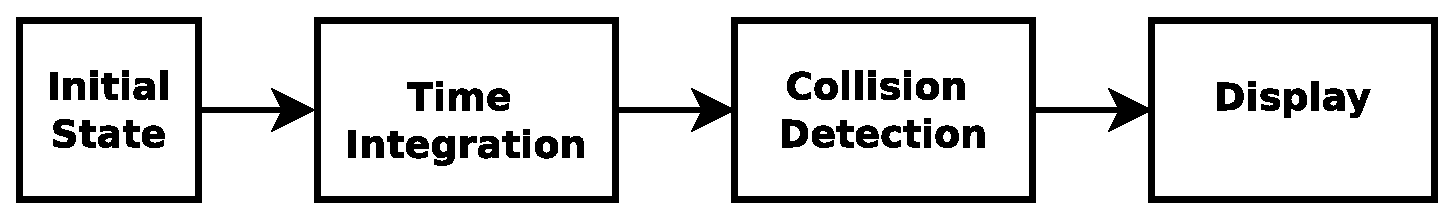
\includegraphics[width=.95\textwidth]{simulation_pipeline2.eps}}
            \only<2>{ 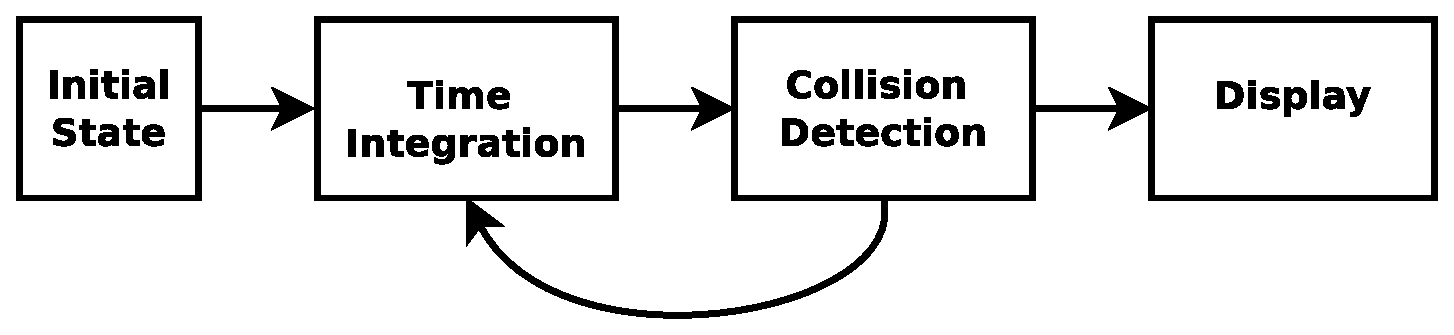
\includegraphics[width=.95\textwidth]{simulation_pipeline3.eps}}
            \only<3>{ 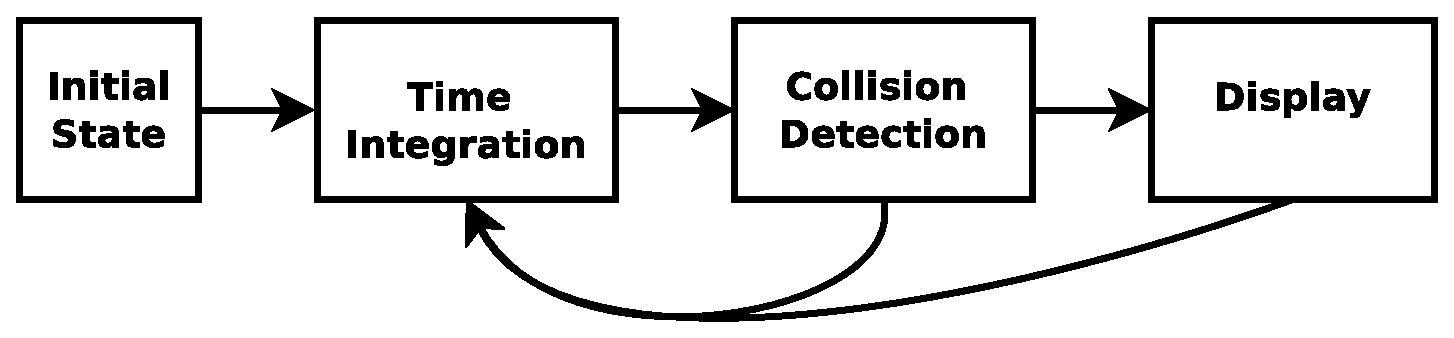
\includegraphics[width=.95\textwidth]{simulation_pipeline4.eps}}
            \only<4->{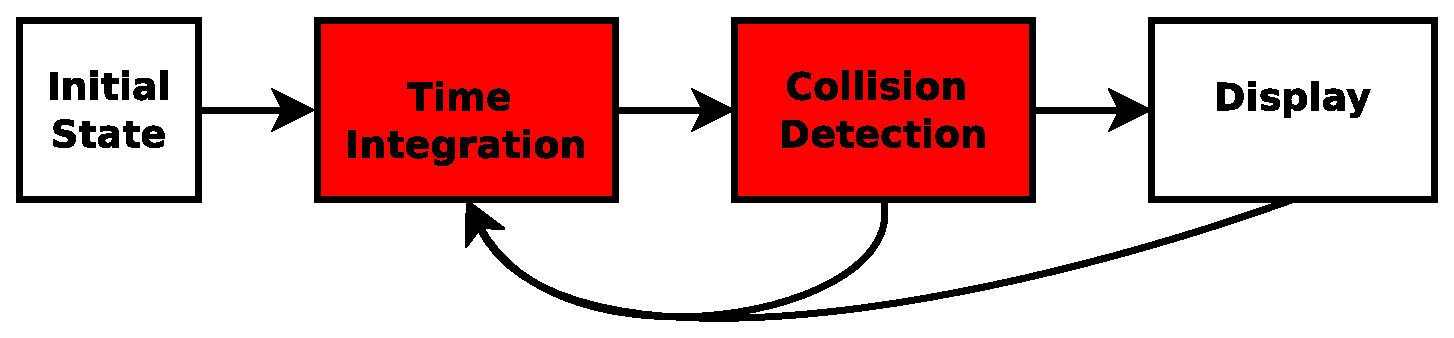
\includegraphics[width=.95\textwidth]{simulation_pipeline5.eps}}
        }
    \end{block}
    \pause
    \pause
    \pause
    \pause
    \begin{alertblock}{Sofa \cite{Allard07SOFA,Nesme09Preserving,Faure11Sparse}}
        \begin{columns}
            \column{.75\textwidth}
            \begin{itemize}[<+->]
                \item Scientific purpose $\Rightarrow$\alert{Precise}
                \item Surgery training $\Rightarrow$\alert{Interactive} 
                \item \alert{Abstract} simulation Framework
                \item Combine any implementation for each step
                \item Very complex class tree
            \end{itemize}
            \column{.2\textwidth}
            
\includegraphics[width=.9\textwidth]{sofa.png}
        \end{columns}
    \end{alertblock}
\end{frame}

\begin{frame}{Previous parallelization of Sofa}
    \begin{itemize}[<+->]
        \item Everton Hermann \cite{Hermann10Simulations} \\
            \begin{itemize}
                \item Parallelization between objects using Kaapi
                \item Good speedup (15 using 16 CPUs), better with GPUs
                \item Not used in recent Sofa version 
            \end{itemize}
        \item Julio Toss \cite{Toss12New}
            \begin{itemize}
                \item Works on algorithms out of Sofa then incorporate them
                \item Ongoing work
            \end{itemize}
        \item Current version openmp \#pragma for
    \end{itemize}
    \pause
    \begin{alertblock}{My approach}
        \begin{itemize}
            \item Focus on Sofa 
            \item \alert{Identify the performances issues}
            \item Find a suitable way to fix them
        \end{itemize}
    \end{alertblock}

\end{frame}

\newsection{Analysis}

\begin{frame}{First Analysis}
    \begin{block}{Methodology}
        \begin{itemize}
            \item Performances counter using Likwid \cite{Treibig10LIKWID}
            \item Analysis at a global level (wrapper mode)
            \item Analysis at a local level (marker mode)
            \item Counters for all cache level, memory, Cycles per instructions
            \item Performance metrics from Sofa (Simulation time, FPS)
            \item 4 representative scenes
        \end{itemize}
    \end{block}
    \pause
    \begin{exampleblock}{First results}
        \begin{itemize}
            \item Hundred of plots
            \item Lot of work to correlate them / keep only the interesting ones
        \end{itemize}
    \end{exampleblock}
\end{frame}

\begin{frame}{Results}

    \only<1>{\includegraphics[width=0.9\textwidth]{img/Runtime_ratio1.png}}
    \only<2>{\includegraphics[width=.9\textwidth]{img/memory_traffic_loc2.png}}
    \only<3->{\includegraphics[width=.9\textwidth]{img/memory_traffic_loc1.png}}
    \only<4>
    {
        \begin{textblock}{14}(1,7)
            \begin{alertblock}{First conclusions}
                \begin{itemize}
                    \item Maybe a problem of false sharing
                    \item We need more informations
                \end{itemize}
            \end{alertblock}
        \end{textblock}
    }
\end{frame}

\begin{frame}{Advanced tools}
    \begin{itemize}
        \item Vtunes \cite{Reinders05VTune}
        \item HPCToolkit \cite{Adhianto10HPCTOOLKIT}
        \item Paraver \cite{Pillet95PARAVER}
        \item MemProf \cite{Lachaize12MemProf}
        \item \dots
    \end{itemize}
    \pause
    \begin{alertblock}{Limitations}
        \begin{itemize}
            \item Complex to use
            \item Focus on the architecture or on the runtime (MPI, etc.)
            \item Most problems come from the memory
            \item We need a different kind of tools
        \end{itemize}
    \end{alertblock}
\end{frame}

\begin{frame}{Designing new tool}
    \begin{itemize}[<+->]
        \item Analysing the memory usage \cite{Beniamine13Cartographier}
        \item Detect patterns (non)-linear acces, high pressure on small set of data \dots
        \item Instrumentation is slow, other methods (IBS ?)
        \item Lot of data, need a suitable tool for visualisation \cite{Pagano13Trace,Dosimont14Trace}
    \end{itemize}
\end{frame}

\newsection{Conclusions}

\newcounter{finalframe}
\setcounter{finalframe}{\value{framenumber}}
%Last numbered frame go here

\begin{frame}{Original approach}
    \todo{blabla}
\end{frame}



%=============================================================================

%=============================================================================
%Uncomment next lines for uncounted backup slides & biblio
\newHsection{Bibliography}
\setboolean{sectiontoc}{false} 
%
\bibliographystyle{apalike} 
\bibliography{presentation}

%========================= Backup slides =====================================
%\newsection*{Hidden slides}
%put this line before each frame
%\setcounter{framenumber}{\value{finalframe}}

%=============================================================================
\end{document}


